\documentclass[11pt,a4paper]{article}

% --------------------------------------------------
% FORMATTING REQUIREMENTS
% --------------------------------------------------

\usepackage[
    top=1.5cm,
    bottom=1.5cm,
    left=2cm,
    right=2cm
]{geometry}

\usepackage[T1]{fontenc}
\usepackage[utf8]{inputenc}
\usepackage{amsmath}
\usepackage{svg}

%\usepackage{setspace}
%\singlespacing

\usepackage{graphicx}
\usepackage{booktabs}
\usepackage{longtable}
\usepackage{array}
\usepackage{enumitem}
\usepackage{caption}
\usepackage{pdflscape}
\usepackage{float}
\usepackage{xcolor}
\usepackage{hyperref}
\usepackage{csquotes}

% Gantt chart
\usepackage{pgfgantt}

% Bibliography
\usepackage[
    backend=biber,
    style=authoryear,
    maxbibnames=99
]{biblatex}

\addbibresource{isotopes.bib}

%\setlength{\parskip}{0.5em}
%\setlength{\parindent}{0pt}

\title{Bolin}
\author{Agnieszka Żaba}

\begin{document}
\section{Requirements}
Detailed description \textbf{in English}, including the following information: 

\begin{enumerate}
\item scientific goal of the project (description of the problem to be solved, research questions and hypotheses); 
\item significance of the project (state of the art, justification for tackling a specific scientific problem,
    justification for the pioneering nature of the project,
    the impact of the project results on the development of the research field and scientific discipline); 
\item concept and work plan (general work plan, specific research goals, results of preliminary research,
    a research work programme, e.g. a Gantt chart, including milestones, risk analysis); 
\item research methodology (underlying scientific methodology, methods, techniques and research tools,
    methods of results analysis, equipment and devices to be used in research); 
\item composition and qualifications of the research team, including (if applicable) achievements
    of the co-investigators named in the proposal; 
\item project literature (a reference list for publications included in the project description,
    with full bibliographic data). 
\end{enumerate}
Recommended formatting: top-bottom margins: at least 1.5 cm, left-right margins: at least 2 cm, font: Times New Roman or equivalent, font size: at least 11, interline: single. 

\subsection{evaluation criteria}
A. PROJECT ASSESSMENT (80\%)
SCIENTIFIC QUALITY – scientific relevance, importance, originality and novelty of
research or tasks to be performed; relevance of the methodology and work plan in
relation to the scientific objectives of the project, including (if applicable) appropriate
integration of sex and/or gender dimension in the project’s content; the scientific
quality of the project should be evaluated in an international context.
FEASIBILITY – the work plan and the methodology in relation to achieving the
proposed objectives within the given timeframe; risk management plan; the
composition and qualifications of the research team, including (if applicable) the
achievements of the research team members already named in the proposal
relevant to the project tasks; allocation of the research tasks; research facilities and
equipment; international cooperation (if any); other factors affecting the feasibility of
the project.
POTENTIAL IMPACT – the potential for impact of the project results and for high-
quality scientific publications and other research outputs of the project; the potential
impact of the project should be evaluated within an international context, taking into
account the specifics of the research field and the variety of forms of impact and
output.
SCORING
5 Excellent project with no significant weaknesses.
4 Very good project with minor weaknesses.
3 Good project with moderate weaknesses.
2 Mediocre project with major weaknesses.
1 Weak project with numerous major weaknesses.
0 Project with critical structural flaws / Project cannot be assessed due to
incomplete information / Project has not been prepared in a reliable manner /
Project does not meet the criterion of basic research8 / Project lacks a scientific
character.

\section{keywords}
Proposition for name:
particle resolved, droplet
Isotopic Composition Evolution
Simulation Evolution of Isotopic Composition 
Isotopic Closure Atmosphere
Ice Liquid Vapor
Isotopic Fractionation
Water Stable Isotopologues
Cloud Using Bolin number for Isotopic Closure
Applicability of the Bolin number to Isotopic Fractionation
Ice Liquid Vapour fractionation Oxygen and Hydrogen
Stable Isotopic Composition
BOLIN, CLOUD, ISOTOPE, OXYGEN, WATER, VAPOUR, ATMOS, ICE, 
Isotopic Fractionation with Bolin number for Aerosol-Cloud Closure
Aerosol-Cloud Isotopic evolution
Bolin number, isotopic fractionation, supersaturation, mixed phase clouds, what isotopes we are considering

BASIC
Bolin number Applicability in Simulations of Isotopic Composition
FIBON - Fractionation of Isotopes with BOlin Number
BINARY, BOUNDARY
Bolin number 

Keywords:

stabilne izotopy wody, frakcjonowanie izotopowe, mikrofizyka chmur, chmury mieszanej fazy, modelowanie z rozdzielczością cząstek, metoda superkropelek, modelowanie atmosfery, oddziaływania aerozol-chmura
stable water isotopes, isotopic fractionation, cloud microphysics, mixed-phase clouds, particle-resolved modelling, super-droplet method, atmospheric modelling, aerosol-cloud interactions



\section{Student oportunity}
In the grant I would be happy to have a co-investigator. 
Student during Bachelor or Masters - I don't have requirements here.
It should be good enough for the student to have possibility to progress their thesis.
The studies must be in one of the following topics: physics, computer sciences, mathematics.
The responsibility would be a creation of the simple (but not trivial) model contained in one notebook 
which will be sufficient to simulate isotopic composition.
Programming abilities needed.
Target programming language: Python, Julia. 
Maybe with visualisations? 


%----------------------------------------------------%
%       REMEMBER!!!
%----------------------------------------------------%
\section{Remember to include}
\begin{itemize}
    \item What is isotopic fractionation (maybe graphics)
    \item Three isotopes as novelty, particle based models isotopic enabled
    \item Presentation of results (important part of a grant)
    \item Bolot analysis
    \item what is new, what is the improvement
\end{itemize}

Citations:
Craig (1961), Dansgaard (1964), Majoube (1971), Merlivat (1978), Merlivat \& Jouzel (1979),
Horita \& Wesolowski (1994), Horita et al. (2008), Stewart (1975), Friedman et al. (1962),
Beard \& Pruppacher (1971), Pruppacher \& Rasmussen (1979), Graf et al. (2019),
De Szoeke et al. (2024), Jouzel (1986), Hiron \& Flossmann (2020), Galewsky et al. (2016),
Gat (1996), Noone (2012), Blossey \& Kuang (2010), and Pruppacher \& Klett (2010).


\section{Fundamentals of Stable Water Isotope Hydrology}
\begin{itemize}
    \item \textbf{Craig (1961)} -- Global Meteoric Water Line (GMWL); foundation of precipitation isotope studies.
    \item \textbf{Dansgaard (1964)} -- Controls on stable isotopes in precipitation; temperature and rainout effects.
    \item \textbf{Merlivat \& Jouzel (1979)} -- Climatic interpretation of the d-excess parameter.
    \item \textbf{Gat (1996)} -- Classic review of oxygen and hydrogen isotopes in the hydrologic cycle.
    \item \textbf{Gat (2010)} -- Comprehensive isotope hydrology textbook.
    \item \textbf{Galewsky et al. (2016)} -- Modern review of atmospheric water-vapor isotopes.
    \item \textbf{Noone (2012)} -- Integration of isotope observations and modeling.
    \item \textbf{Jouzel et al. (2013)} -- Water isotopes as tracers of moisture sources.
\end{itemize}

\section{Equilibrium Isotope Fractionation}
\begin{itemize}
    \item \textbf{Majoube (1971)} -- Standard equilibrium liquid--vapor fractionation factors.
    \item \textbf{Horita \& Wesolowski (1994)} -- Updated equilibrium fractionation factors over a wide temperature range.
    \item \textbf{Merlivat \& Nief (1967)} -- Ice--vapor fractionation factors.
    \item \textbf{Jouzel (1986)} -- Isotopic fractionation during cloud processes.
    \item \textbf{Kakiuchi (2000)} -- Molecular partitioning of isotopologues between phases.
\end{itemize}

\section{Kinetic Fractionation and Evaporation Theory}

\begin{itemize}
    \item \textbf{Horita et al. (2008)} -- Comprehensive review of the Craig--Gordon evaporation model.
    \item \textbf{Merlivat (1978)} -- Molecular diffusivities of water isotopologues.
    \item \textbf{Hellmann \& Harvey (2020)} -- First-principles diffusivity ratios.
    \item \textbf{Merlivat \& Coantic (1975)} -- Isotope transfer at the air--water interface.
    \item \textbf{Gonfiantini et al. (2020)} -- Wind effects on isotope fractionation during evaporation.
    \item \textbf{Pierchala et al. (2022)} -- Triple-isotope diffusion-induced fractionation.
\end{itemize}

\section{Raindrop Evaporation and Below-Cloud Processes}
\begin{itemize}
    \item \textbf{Stewart (1975)} -- Classical treatment of isotope fractionation in falling raindrops.
    \item \textbf{Friedman et al. (1962)} -- Water-vapor exchange between droplets and surrounding air.
    \item \textbf{Booker (1965)} -- Experimental isotope exchange between droplets and vapor.
    \item \textbf{Cappa et al. (2003)} -- Isotopic fractionation during evaporation.
    \item \textbf{Graf et al. (2019)} -- Modern framework for below-cloud isotope effects.
    \item \textbf{Graf (2017)} -- Detailed analysis of below-cloud isotope processes.
    \item \textbf{De Szoeke et al. (2024)} -- Simple isotope-enabled hydrometeor evaporation model.
    \item \textbf{Worden et al. (2007)} -- Global significance of rain evaporation.
\end{itemize}

\section{Cloud Microphysics and Droplet Growth}
\begin{itemize}
    \item \textbf{Pruppacher \& Klett (2010)} -- Standard reference for cloud microphysics.
    \item \textbf{Köhler (1936)} -- Köhler theory and cloud droplet activation.
    \item \textbf{Howell (1949)} -- Condensational growth of cloud droplets.
    \item \textbf{Carstens (1979)} -- Review of droplet growth by condensation.
    \item \textbf{Jensen \& Nugent (2017)} -- Growth on giant sea-salt aerosol particles.
    \item \textbf{Mason (1951)} -- Classical condensation experiments.
    \item \textbf{Tsuji (1950)} -- Supersaturation and cloud particle growth.
    \item \textbf{Fahandezh Sadi et al. (2026)} -- Supersaturation fluctuations and haze-cloud interactions.
\end{itemize}
\section{Raindrop Dynamics and Evaporation Physics}
\begin{itemize}
    \item \textbf{Gunn \& Kinzer (1949)} -- Terminal velocity of water droplets.
    \item \textbf{Kinzer \& Gunn (1951)} -- Evaporation and thermal relaxation of falling drops.
    \item \textbf{Beard \& Pruppacher (1971)} -- Evaporation rates of small falling droplets.
    \item \textbf{Pruppacher \& Rasmussen (1979)} -- Evaporation rates of large falling droplets.
    \item \textbf{Tsuji (1950)} -- Early evaporation-rate calculations.
    \item \textbf{Loftus \& Wordsworth (2021)} -- Modern treatment of falling-drop physics.
\end{itemize}

\section{Cloud Isotope Microphysics}
\begin{itemize}
    \item \textbf{Jouzel (1986)} -- Foundational review of isotopes in cloud physics.
    \item \textbf{Hiron \& Flossmann (2020)} -- Bin-resolved cloud isotope microphysics model.
    \item \textbf{Federer et al. (1982)} -- Isotope cloud model for hail formation.
    \item \textbf{Jouzel et al. (1975)} -- Isotopic observations in hail.
    \item \textbf{Lamb et al. (2017)} -- Laboratory measurements of ice deposition fractionation.
    \item \textbf{Nelson (2011)} -- Theory of isotopic fractionation on ice crystals.
    \item \textbf{Webster \& Heymsfield (2003)} -- Isotope constraints on cloud dehydration.
    \item \textbf{KleinStern et al. (2026)} -- Laboratory cloud-chamber isotope experiments.
\end{itemize}

\section{Isotope-Enabled Atmospheric Modeling}

% Numerical representation of isotopes in clouds and the water cycle.

\begin{itemize}
    \item \textbf{Joussaume et al. (1984)} -- First isotope-enabled GCM.
    \item \textbf{Hoffmann et al. (1998)} -- ECHAM isotope module.
    \item \textbf{Hoffmann et al. (2000)} -- Review of isotope GCM developments.
    \item \textbf{Blossey \& Kuang (2010)} -- Cloud-resolving isotope simulations.
    \item \textbf{Bolot et al. (2013)} -- Isotopes in convective updrafts.
    \item \textbf{Lee et al. (2007)} -- Prediction of precipitation isotopes using GCMs.
    \item \textbf{Wei et al. (2018)} -- Coupled isotope LES-cloud system.
    \item \textbf{Haese et al. (2013)} -- Coupled atmosphere-land isotope model.
    \item \textbf{Eichinger et al. (2015)} -- Isotope-enabled EMAC model.
    \item \textbf{Xu et al. (2012)} -- Isotope-enabled ocean model.
\end{itemize}

\section{Atmospheric Water Vapor Isotopes}
\begin{itemize}
    \item \textbf{Frankenberg et al. (2009)} -- Controls on lower-tropospheric HDO/H$_2$O.
    \item \textbf{Rozanski \& Sonntag (1982)} -- Vertical isotope profiles of atmospheric vapor.
    \item \textbf{Johnson et al. (2001)} -- Stratospheric water isotopes and transport.
    \item \textbf{Moyer et al. (1996)} -- Troposphere-stratosphere exchange.
    \item \textbf{Lossow et al. (2011)} -- Satellite HDO validation.
    \item \textbf{Wen et al. (2008)} -- Continuous vapor isotope measurements.
\end{itemize}

\section{Analytical Methods and Calibration}
\begin{itemize}
    \item \textbf{Craig (1957)} -- Isotopic standards.
    \item \textbf{Gonfiantini (1978)} -- Stable isotope measurement standards.
    \item \textbf{Gröning (2011)} -- Calibration and uncertainty estimation.
    \item \textbf{Tremoy et al. (2011)} -- Caveats in CRDS measurements.
    \item \textbf{Weng et al. (2020)} -- Mixing-ratio corrections for CRDS systems.
\end{itemize}

\section{Supporting Atmospheric Physics References}
\begin{itemize}
    \item \textbf{Seinfeld \& Pandis (2016)} -- Atmospheric chemistry and physics reference.
    \item \textbf{Shima et al. (2009)} -- Super-droplet method.
    \item \textbf{Shipway \& Hill (2012)} -- Warm-rain parameterization comparison.
    \item \textbf{Morrison et al. (2026)} -- Virtual cloud physics laboratory.
\end{itemize}

%----------------------------------------------------%
%       SCIENTIFIC OBJECTIVE
%----------------------------------------------------%

\section{Scientific Objective of the Project}
Panel ST10: Earth sciences

Earth system science, atmospheric sciences, climatology, geochemistry, geodesy, geoecology, geophysics,
physical geography, geoinformatics, planetary geology, pedology, mining, chemical and physical oceanology,
environmental protection
scientific goal of the project (description of the problem to be solved, research questions and hypotheses)

% Meaning of isotopologue studies in the Earth sciences including atmospheric sciences and Earth system science.
% I could mention here also climatology and geochemistry/geophysics
Water stable isotopologues serve as the natural tracers in the global hydrological
cycles of the Earth.

% From chat - introduction:
The isotopic composition of atmospheric water constitutes one of the most informative
tracers of processes occurring within the Earth system.
Stable water isotopes are widely used in atmospheric sciences, climatology, and hydrology
to investigate moisture sources, transport pathways, cloud microphysics,
and interactions between the atmosphere and the hydrological cycle.
The interpretation of isotopic observations relies on an accurate understanding
of isotopic fractionation processes governing the evolution of water vapor
and liquid water in natural environments.

The primary objective of the proposed project is to develop a mathematically rigorous
and physically consistent
framework describing isotopic fractionation during diffusional processes
involving stable water isotopes.
The project aims to formulate, analyze, and implement a process-based model capable
of reproducing
the evolution of isotopic composition in water droplets and the surrounding environment under
varying thermodynamic conditions.

A further objective is to evaluate the predictive capability
of the developed framework through systematic
comparison with experimental and observational datasets.
By confronting theoretical predictions with measurements, the project will assess the validity
of current assumptions regarding kinetic fractionation.

% Important here
The expected outcome is an improved understanding of diffusional isotope fractionation mechanisms
and the development of a reproducible modeling framework that can support future applications of
stable water isotopes in atmospheric research, climate studies, and Earth system science.

Objective:
To develop and validate a mathematically rigorous framework describing isotopologue-specific diffusional
fractionation and to determine how differences in isotopologue transport properties can be used to quantitatively
infer the dynamics of coupled phase-change and transport processes in the atmosphere.

Although the proposed framework is developed for stable water isotopes, the underlying mathematical
formulation is sufficiently general that it may be extended to other systems involving simultaneous
transport or transformation of multiple species characterized by distinct diffusivities or kinetic properties.

% end
Not only studying HDO, H2 18O but also water molecule with substituted Oxygen-17 became more useful thanks to the
advancements in the measurements - using Ring Down Cavity it is possible to measure isotopic content of this isotopologue.
The relations between those three isotopologues are currently researched. 



Advances in modeling isotopic composition of water.
Questions: {\color{red}TODO}
\begin{enumerate}
    \item Is this concept valid and what are its limitations? When can be used?
    \item How to use it? It is not scientific question .. 
    \item Isotopic closure
    \item What models can we compare with? I thinkthis should be in the next steps
\end{enumerate}

Hypothesis is that we can close the system and have information top to bottom, bottom to top
That we can predict and recreate cloud information from precipitation and from ice cores
(preserved isotopic composition).

%----------------------------------------------------%
%       SIGNIFICANCE
%----------------------------------------------------%

\section{Significance of the Project}
significance of the project (state of the art, justification for tackling a specific scientific problem,
justification for the pioneering nature of the project,
the impact of the project results on the development of the research field and scientific discipline)

% Other models like (global, climatology, Erth): 
% ECHAM-wiso :Max Plank, global climate model https://www.dlr.de/en/pa/research-transfer/research-infrastructure/models-1/echam)
% iCAM: isotope enabled Community Atmosphere model (D, Oxygen-18), NCAR
% LMDZ-iso Laboratoire de Météorologie Dynamique Zoom: atmospheric general circulation model (paleoclimate) D, Oxygen-18
% CLoud resolving CRM, LES isotope models
% SAM - University of Chicago
% PartMC-MOSAIC - Illinois
% MIMICA - Stockholm 
The theoretical foundations of isotopic fractionation in clouds are well established through
the concepts of equilibrium and kinetic fractionation and their application to atmospheric processes
(Dansgaard, 1964; Jouzel and Merlivat, 1984).
A major advance was provided by Bolot et al. (2013),
who developed a unified framework describing isotopic evolution in convective updrafts,
including supersaturation effects, isotopic re-equilibration, mixed-phase processes,
and alternative glaciation pathways.
Their work demonstrated that isotopic observations can constrain key
cloud microphysical parameters such as supersaturation, supercooled liquid water content,
and glaciation temperature.
In parallel, particle-resolved cloud models based on the Super-Droplet Method have become
state-of-the-art tools for representing aerosol-cloud interactions and
mixed-phase cloud evolution with unprecedented physical realism (Shima et al., 2009; Arabas and Shima, 2017).
However, isotopic fractionation has not yet been systematically incorporated into particle-resolved cloud microphysics.
Consequently, the detailed isotopic signatures of individual droplets and ice particles,
as well as the consistency of isotope evolution with conservation laws and thermodynamic equilibria,
remain largely unexplored.
The proposed project addresses this gap by developing a mathematically
rigorous isotope-enabled super-droplet framework for mixed-phase clouds,
bridging isotope process modeling and particle-resolved cloud microphysics.

Stable isotopes of water 
provide unique information on cloud formation, phase transitions, and atmospheric moisture transport.
Measurements of isotopic composition in vapor, cloud water, precipitation and ice crystals
have become an important tool for investigating microphysical processes that cannot be directly observed.

Theoretical descriptions of isotope fractionation are well established.
Equilibrium fractionation during phase transitions is described by thermodynamic fractionation factors,
whereas kinetic fractionation accounts for non-equilibrium effects associated
with diffusion and supersaturation.
Classical frameworks include Rayleigh distillation theory and its extensions
to mixed-phase and non-equilibrium cloud systems.

Despite substantial progress in isotope measurements, interpretation of observations remains
limited by the availability of physically consistent numerical models capable
of representing isotope evolution at cloud-process scales.


Existing isotope-enabled cloud models generally:
\begin{itemize}
\item use bulk representations of cloud water,
\item neglect individual particle histories,
\item focus primarily on liquid-phase processes,
\item rarely include multiple isotopes simultaneously,
\item seldom consider mathematically rigorous verification of conservation properties and thermodynamic consistency.
\end{itemize}
As a result, there currently exists no broadly available framework capable of:
\begin{enumerate}
\item tracking isotopic composition of individual super-droplets,
\item representing coupled liquid-water and ice fractionation,
\item simulating multiple isotopes simultaneously,
\item verifying conservation laws and thermodynamic consistency,
\item comparing results directly with modern in-cloud isotope measurements.
\end{enumerate}
This gap limits the ability of the atmospheric science community to exploit isotopic observations
for understanding cloud microphysics.

Stable isotope fractionation has been studied in theoretical, parcel, and bin-resolved cloud models,
while particle-resolved super-droplet models have become state-of-the-art tools for cloud microphysics.
However, these two developments have remained largely disconnected.
At present, no open and mathematically verified framework exists for simulating isotopic evolution
within a super-droplet model capable of representing aerosol-cloud interactions and mixed-phase cloud processes.
Consequently, the potential of isotopic observations to
constrain particle-resolved cloud microphysics remains largely unexplored.

The project aims to develop, analyse, implement, and validate an isotope-enabled extension
of PySDM that allows simulation of stable water isotopes in particle-resolved cloud microphysics,
including liquid-water and ice processes and simultaneous treatment of multiple isotopes.


\subsection{
my previous work on the isotopes
}



%%%%%%%%%%%%%%%%%%%%%%%%%%%%%%%%%%%%%%%%%%%%%%%%%%%%%
% 3. RESEARCH CONCEPT AND WORK PLAN
%%%%%%%%%%%%%%%%%%%%%%%%%%%%%%%%%%%%%%%%%%%%%%%%%%%%%

\section{Research Concept and Work Plan}

Describe the general concept and logic of the project.

Tasks/objectives: 
\begin{enumerate}
    \item\label{itm-maths} Mathematical modeling and analysis: theoretical consistency
    \item\label{itm-code} Implementation including water-ice interactions, Research Software Engineering
        - simplified model ready to use (is it needed in the community?)
    \item\label{itm-data} Comparison with measurements data!
    \item\label{itm-models} \color{red} Comparison with other models (here possibility to make collaborations)
\end{enumerate}

\subsection{Task: \ref{itm-maths}}
Mathematical description of the assumptions of the models with approximation analysis
Verification of mathematical consistency including dimensional analysis, conservation laws.
Behavior analysis: What happens when approaching RH=1?
What happens when isotopic composition of the phases is achieved?
Are theoretical equilibria (thermodynamics and isotopic) satisfied?
What happens for multiple isotopes at the same time?
Limitations of this approach.

Existence of the solution
Stability of solutions under small perturbations

Physics: Rayleigh Distillation, equilibrium and kinetic fractionation
mixed-phase cloud models
Does your equation reduce to standard Rayleigh behavior in the appropriate limit?
Does it reproduce equilibrium fractionation when diffusion effects vanish?
Does it recover kinetic fractionation formulas when cloud microphysics dominates?

\subsection{Task: \ref{itm-code}}
Preliminary: The implementation will be developed within the established PySDM framework, ensuring
compatibility with existing cloud microphysics modules and facilitating reuse by the community.
he PySDM environment will serve as the primary computational framework, extended here to include water–ice interactions and multi-isotopologue tracking.

Adding multiple isotopes analysis in the same time.
RSE: preparing Jupyter Notebook in Python and Julia self-containing all the code needed
to run simulation with isotopic fractionation.

Including test controlled scenarios, unit tests, dimensional analysis of the code
Adiabatic ascent, pure condensation, Constant temperature, polluted and pristine scenario, cloud system cloud, open-system cloud

With this we can compare: maximum error?
Fractionation ratio error? 

Sensitivity analysis of the parameters: temperature, relative humidity, supersaturation, droplet size dristribution, ice fraction, condensation rate, 
initial isotopic composition of the vapor and liquid, 
Sensitivity of the approximations: molecular vs atomic, one isotopologue vs many at the same time
Methods: ...



\subsection{Task: \ref{itm-data}}
Comparison with the data from CAESAR Campaign with collaboration with Elise Rosky.
Preparation for the specific scenario.
Measurements consist of temperature, altitude, isotopic composition of liquid and vapor, droplet size distribution.
Starting with data below the cloud and simulating parcel we can compare resulting droplet distribution and isotopic content.
Uncertainty propagation (?)
Cloud isotope measurements and fractionation coefficients
Approaches: Monte Carlo ensembles, Bayesian parameter estimation, analytical error propagation when possible.

in-cloud isotope measurements, rainwater precipitation isotope measurements
ice crystal isotope observations
laboratory cloud chamber experiments

Correlation, bias, variance explained, residual structure
Ask whether the model predicts realistic behavior under known cloud conditions.


AMS Abstract

The isotopic composition of precipitation and cloud water reflects the history
 of both diffusional and collisional growth of the hydrometeors.
Stable water isotopologues provide valuable insight into the sources and pathways
 of water in the environment, making them natural tracers of the hydrological cycle.
The stable isotopologues considered include $\mathrm{HDO}$, $\mathrm{H_2^{17}O}$ and $\mathrm{H_2^{18}O}$.
Diffusional processes drive isotopic fractionation through both equilibrium
 and kinetic effects, with kinetic fractionation coupled with ventilation
 and saturation dynamics.

In this work, we report on the development of a particle-based
 aerosol-cloud microphysics model that explicitly resolves isotopic fractionation.
The model extends the Super-Droplet Method (SDM) probabilistic approach introduced
 in \cite{2009_Shima_EtAl}.
SDM efficiently represents aerosol-cloud interactions originating from both
 diffusional and collisional processes.
It has favourable computational scaling properties compared with bin-resolved
 microphysics models,
 what results in the ability to track additional particle properties.
Hence, extending particle-based model with e.g. isotopic content in droplets can be
 done without modifications in the model structure or significant additional cost
 for the representation of particle transport.

In the proposed representation of isotopic fractionation processes, each super-droplet
 is assigned with extensive attributes pertaining to its isotopic composition.
While the diffusional dynamics remain unchanged compared to standard SDM formulation,
 additional dynamics are introduced to capture the mass transfers of different
 isotopologues in both liquid and vapor phases.
For computing isotopic fractionation effects we introduce a quantity herein referred
 to as the Bolin number, first proposed conceptually in \cite{1958_Bolin} with the context
 of tritium evolution in precipitation.

The Bolin number is defined as:
$\textbf{Bo} = \frac{\tau_\text{heavy}}{\tau_\text{light}} \approx \frac{\tau_\text{heavy}}{\tau_\text{total}}$,
 where $\tau = \left(\frac{1}{m} \frac{dm}{dt}\right)^{-1}$
 represents the characteristic equilibration timescale of a given water isotopologue.
By defining this number explicitly, the evolution of a heavy isotopologue can be
 inferred from the dynamics of the mass of the light isotopologue (or approximately
 of the droplet total mass).
The use of the Bolin number simplifies model formulation by capturing,
 the efficiency of isotopic fractionation in a single dimensionless value.
It incorporates quantities such as the equilibrium fractionation factor
 $\left(\alpha_\text{eq}\right)$, as well as heat conduction and mass diffusion
 effects (including ventilation), and environmental conditions such as temperature
 and saturation ratio.

In the poster, we report on: (i) the implementation of the triple-isotope
 fractionation dynamics in the open-source cloud microphysics modeling package PySDM,
 and (ii) a revisited theoretical analysis of isotopic ratio evolution in evaporating
 raindrops presented in \cite{1994_Gedzelman_Arnold}.
We extend this analysis to capture the influence of the drop concentration on the
 fractionation efficiency.
In Figure 1, the dynamics of deuterium content in both liquid and vapor phases
 are depicted by examining the dependence of the magnitude of the time derivative
 of the isotopic delta on ambient saturation ratio and the initial isotopic delta
 of the liquid phase.
The figure follows the construction of Fig. 2 in \cite{1994_Gedzelman_Arnold},
 extended here to include a third dimension.
The plots show how the system responds to being forced out of both phase
 and isotopic equilibria.

The developed model provides a practical tool for integrating aerosol–cloud
 interactions with stable-isotope fractionation analyses by combining particle-based
 microphysics modeling with isotopic tracers.
By constraining supersaturation and mixing during entrainment, modeling isotopic
 fractionation enables reconstruction of saturation conditions and cloud processes
 and could help distinguish between inhomogeneous and homogeneous mixing.

Present any pilot studies, preliminary data, proofs of concept, or previous work.

    {\color{red}TODO: plot}
\begin{figure}
    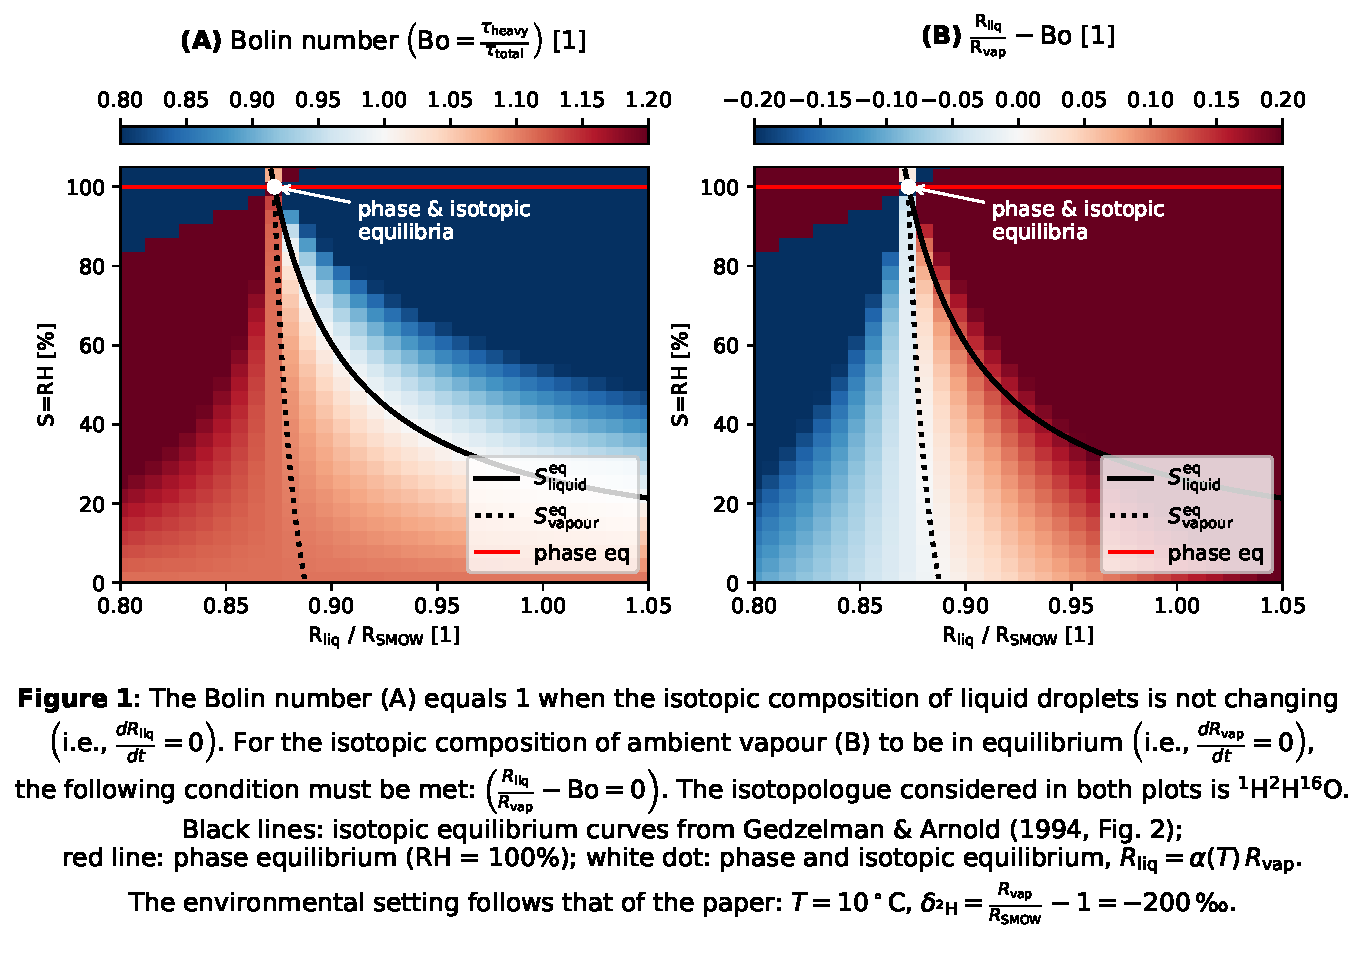
\includegraphics[width=\textwidth]{Bo}
\end{figure}


\subsection*{(A) Previous work: computational framework for isotopic cloud microphysics}
In previous NCN-funded research, I developed and implemented extensions of the PySDM particle-based cloud microphysics
framework enabling quantitative analysis of stable water isotope fractionation in clouds.
The work focused on introducing physically based timescale formulations and analytical representations
of isotopic equilibration processes in cloud droplets.

Specifically, I implemented a set of four physically motivated formulations for isotopic equilibration timescales
($\tau$) based on classical literature (\cite{1958_Bolin}, \cite{1984_Jouzel_Merlivat}(or '75?), \cite{1975_Stewart}),
and diffusion-based derivations from first principles (Fick’s law and Fourier-type analogies).
These formulations were integrated into PySDM as modular Python classes with a unified interface,
enabling systematic comparison of competing theoretical descriptions.

The implementation was accompanied by full software documentation (NumPy/Sphinx style) integrated
into the PySDM documentation system, ensuring usability and reproducibility within the open-source community.
Particular attention was given to dimensional consistency, numerical stability, and clarity of physical assumptions.

\subsection*{(B) Analytical modeling of isotopic fractionation dynamics}
In parallel, I developed an analytical model of isotopic fractionation in cloud systems.
The model describes the evolution of heavy water isotopologues ($\mathrm{HDO}$, $\mathrm{H_2^{17}O}$, $\mathrm{H_2^{18}O}$)
coupled to bulk microphysical evolution of droplets.
A key outcome of this work was the introduction of a dimensionless quantity (the Bolin number),
which relates the {\color{red}characteristic equilibration timescales} of heavy and light isotopologues.
This formulation allows the isotopic evolution problem to be reduced to a compact dimensionless representation
that captures equilibrium and kinetic fractionation regimes within a unified framework.

First implementation of the model was developed within PySDM and validated against theoretical benchmarks,
including the isotopic equilibrium curves presented in \cite{1994_Gedzelman_Arnold}.
Initial results confirmed that the proposed formulation reproduces
expected equilibrium conditions under limiting assumptions.

\subsection*{(C) Model validation}
The initial validation was performed using automated unit tests integrated into GitHub Actions workflows,
ensuring correctness of physical constraints and numerical implementation.
A preliminary comparison with theoretical predictions demonstrated consistency
with established isotopic fractionation theory.

The results were accepted for presentation at the 17th Conference on Cloud Physics 
(AMS Madison Summit 2026),
where the particle-based isotopic microphysics framework and the Bolin number formulation
will be presented to the atmospheric science community.

% IMPORTANT TO STATE WHAT WILL BE NEW! REFINE

\section*{(D) What is new in the proposed project}
Despite these advances, the current framework remains limited in three fundamental aspects:
First, the existing implementation focuses primarily on timescale formulations and simplified isotopic evolution laws,
without a fully consistent treatment of coupled water–ice phase interactions.
Also this approach needs further analysis: in this formulation the Bolin number must remain
positive while we can imagine situation when
changes of mass for heavy and light isotopologue are opposite signs.
Mixed-phase processes, which are essential for realistic cloud systems,
are not yet represented in a unified isotopic framework.

Second, the current model describes isotopic fractionation largely in
a diagnostic or semi-analytical form,
rather than as a fully coupled prognostic system embedded within cloud microphysics.
As a result, feedbacks between microphysical evolution
(condensation, deposition, freezing, riming)
and isotopic composition are not fully resolved.
(We have to think about this)

Third, there is currently no systematic data-constrained validation framework linking
the model to field and laboratory observations across multiple measurement types
(cloud water, vapor, precipitation, and ice phase isotopic composition).

The proposed project addresses these limitations by developing a fully coupled,
physically consistent water–ice isotopic microphysics model, extending the current PySDM-based framework to include:

- explicit mixed-phase cloud processes,
- multi-isotope prognostic evolution in all phases,
- and systematic validation against observational datasets (including CAESAR campaign data and laboratory cloud chamber experiments).





\subsection{Milestones}
Mathematical analysis of constrains
Multiple isotopes simultanuosly resolved

Comparison with measurements (sensitivity, analysis, what is the importance of our approach?)
Validation of the model, analysis on limitations

Ice phase in simulations
Comparison with measurements - contiunuation

\subsection{Risk Analysis}





%%%%%%%%%%%%%%%%%%%%%%%%%%%%%%%%%%%%%%%%%%%%%%%%%%%%%
% 4. RESEARCH METHODOLOGY
%%%%%%%%%%%%%%%%%%%%%%%%%%%%%%%%%%%%%%%%%%%%%%%%%%%%%

\section{Research Methodology}
How it will be conducted?


Methods and Techniques: 
1. Experimental methods: 
  only with collaboration with Elise, work on the new experiment about isotopic composition between ice and vapour (one snowflake)

2. Theoretical methods:
  mathematical analisis of errors

3. Computational: 
 - should I explain here on my programming character? Like what language...

- Data Collection - in separate field

- Data Analysis: Describe analysis procedures and validation methods.

- Research Infrastructure: Describe equipment, laboratory facilities, software, databases,
and other research tools.

- Research Team and Qualifications


\appendix

\clearpage
\printbibliography

\end{document}

